% !TeX spellcheck = en_GB
% !TeX root = ../build/main.tex

\section{Introduction}

\begin{frame}[allowframebreaks]{First Example: The Fibonacci Sequence}
\begin{columns}
\begin{column}{0.3\textwidth}
\begin{figure}
	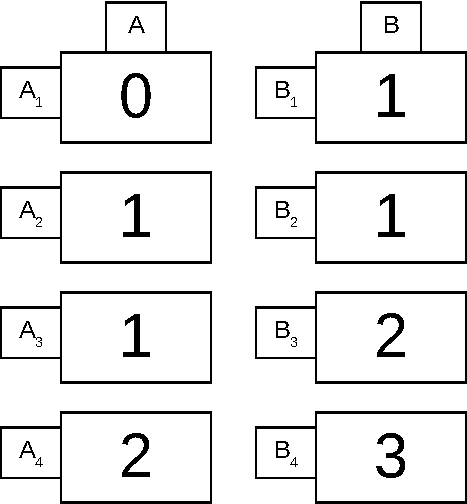
\includegraphics[width=\textwidth]{\zkevmdir/architecture/figures/fibonacci-sequence}
\end{figure}
\end{column}
%\hspace{-1.4cm}
\begin{column}{0.7\textwidth}
\begin{itemize}
\small
\item We can build the Fibonacci state machine with two registries: $A$ and $B$.
\item Then, we have the following relations between the states of these registries:
\begin{align*}
A_{i+1} &= B_i, \\
B_{i+1} &= A_i + B_i,
\end{align*}
for $i \in [5]$.

\item Now, represent these states as polynomials evaluated on the group $H = \{\omega, \omega^2, \omega^3, \omega^4, \omega^5 = 1\}$:
\begin{align*}
A(\omega^i) &= A_i \quad \Longrightarrow \quad A = [0, 1, 1, 2, 3] \\
B(\omega^i) &= B_i \quad \Longrightarrow \quad B = [1, 1, 2, 3, 5]
\end{align*}
for $i \in [5]$.
\end{itemize}
\end{column}
\end{columns}

\begin{columns}
\begin{column}{0.3\textwidth}
\begin{figure}
	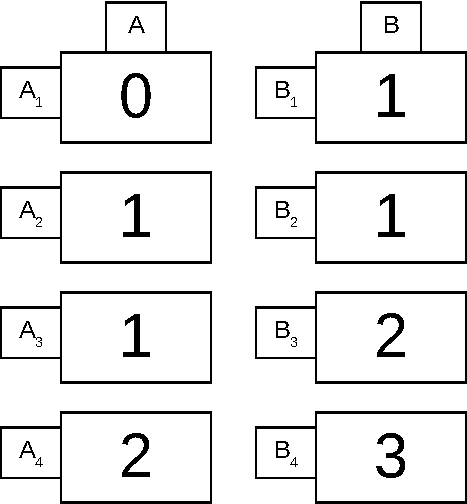
\includegraphics[width=\textwidth]{\zkevmdir/architecture/figures/fibonacci-sequence}
\end{figure}
\end{column}
%\hspace{-1.4cm}
\begin{column}{0.7\textwidth}
\begin{itemize}
\small
\item We can now translate the previous relations to the polynomial setting:
\begin{align*}
A(x\omega) &=  B(x), \\
B(x\omega) &=  A(x) + B(x).
\end{align*}

\item However, this is not completely correct, since when we evaluate in $\omega^5$ we obtain:
\begin{align*}
A(\omega^6) = A(\omega) = 0 &\neq  5 = B(\omega^5), \\
B(\omega^6) = B(\omega) = 1 &\neq  8 = A(\omega^5) + B(\omega^5).
\end{align*}

\item Let's add an auxiliary registry $C$ to solve this problem.
\item To create simple polynomial identities that can can be described as relations between successive points in H, 
we will make the state machine cyclic, that is, to start again in (0,1).
\end{itemize}
\end{column}
\end{columns}

\begin{columns}
\begin{column}{0.4\textwidth}
\begin{figure}
	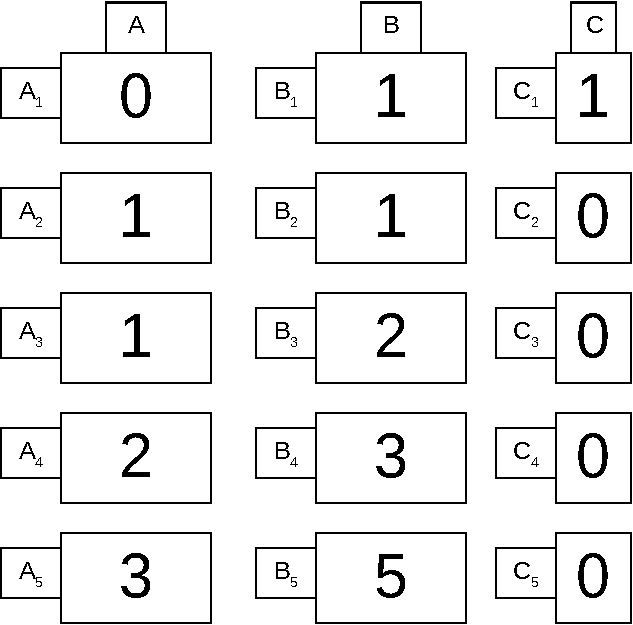
\includegraphics[width=\textwidth]{\zkevmdir/architecture/figures/fibonacci-sequence-aux}
\end{figure}
\end{column}
%\hspace{-1.4cm}
\begin{column}{0.6\textwidth}
\begin{itemize}
\small
\item Similarly to $A$ and $B$, represent the state $C$ as a polynomial evaluated on $H$:
\begin{align*}
C(\omega^i) &= C_i \quad \forall i \in [5] \quad \Longrightarrow \quad C = [1, 0, 0, 0, 0].
\end{align*}
\item With this auxiliary state, we can now fix the polynomial identities as follows:
\begin{align*}
A(x\omega) &=  B(x)(1 - C(x\omega)), \\
B(x\omega) &=  (A(x) + B(x))(1 - C(x\omega)) + C(x\omega).
\end{align*}
%\begin{align*}
%C(x)A(x) &= 0, \\
%C(x)(B(x) - 1) &= 0, \\
%A(x\omega) &=  B(x), \\
%B(x\omega) &=  A(x) + B(x).
%\end{align*}

Notice that now, when $x = w^5$:

$A(Xw) = A(w^6) \neq B(X)$ ; $A(Xw) = A(w^6) = 0$.

$B(Xw) = B(w^6) \neq A(X)+B(X)$ ; $B(Xw) = B(w^6) = 1$.
\end{itemize}
\end{column}
\end{columns}
\end{frame}



%TODO: Do it step by step (limiting only moving one state to another and blabla) and better explanations

%TODO: Generalize it to multiple states in parallel
\begin{frame}[allowframebreaks]{Starting from the Basics: Move State Machine}
\vspace{-0.3cm}
\begin{figure}
	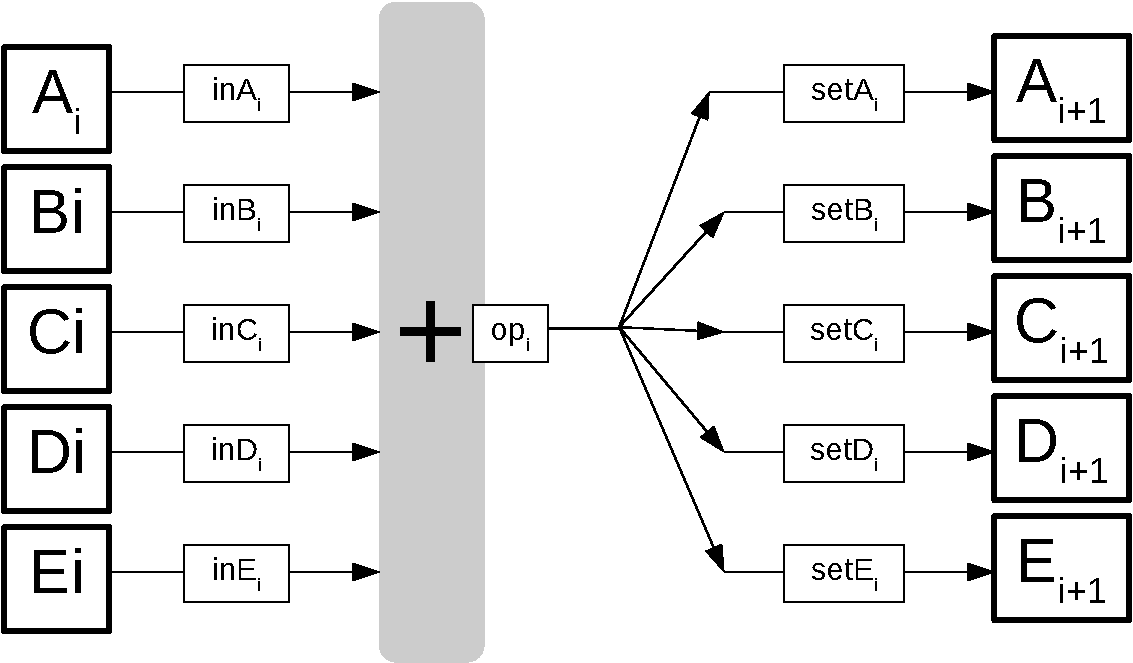
\includegraphics[width=0.8\textwidth]{\zkevmdir/architecture/figures/main-state-machine-simplified}
\end{figure}

\begin{itemize}
\item We have used the following notation:
\begin{enumerate}[a)]
\item \textbf{inX}: $1$ or $0$ depending if the state $X_i$ is included in the sum or not.

\item \textbf{op}: The resulting operation between the included states.

\item \textbf{setX}: $1$ or $0$ depending if one state (or a combination or more) will be moved into $X_{i+1}$.
\end{enumerate}
 
\item The relations between the states of the registries can be expressed as follows:
\begin{align*}
\op_i &= A_i \cdot \inp A_i + B_i \cdot \inp B_i + C_i \cdot \inp C_i + D_i \cdot \inp D_i + E_i \cdot \inp E_i, \\
A_{i+1} &= \set A_i \cdot (\op_i - A_i) + A_i, \\
B_{i+1} &= \set B_i \cdot (\op_i - B_i) + B_i, \\
C_{i+1} &= \set C_i \cdot (\op_i - C_i) + C_i, \\
D_{i+1} &= \set D_i \cdot (\op_i - D_i) + D_i, \\
E_{i+1} &= \set E_i \cdot (\op_i - E_i) + E_i.
\end{align*}
\end{itemize}
\end{frame}










\begin{frame}[allowframebreaks]{How to Encode the Move State Machine}
\begin{itemize}
\small
\item Let's assume that we want to perform the following instructions:
\begin{align*}
\mathbf{MOV}~B, A \quad \mathbf{MOV}~C, D \quad \mathbf{MOV}~A, D \quad \mathbf{MOV}~E,B.
\end{align*}
\end{itemize}
\[
%\begin{array}{|c|}
%\hline
%\mathbf{Inst.~Name} \\ \hline
%MOV \quad B, A \\ \hline
%MOV \quad C, D \\ \hline
%MOV \quad A, D \\ \hline
%MOV \quad E, B \\ \hline
%\end{array}
%\hspace{0.1cm}
\begin{array}{|c|}
\hline
\mathbf{Position} \\ \hline
0 \\ \hline
1 \\ \hline
2 \\ \hline
3 \\ \hline
\end{array}
\hspace{0.1cm}
\begin{array}{|c|c|c|c|c|c|c|c|c|c|}
\hline
\inp A & \inp B & \inp C & \inp D & \inp E & \set A & \set B & \set C & \set D & \set E \\ \hline
1 & 0 & 0 & 0 & 0 & 0 & 1 & 0 & 0 & 0 \\ \hline
0 & 0 & 0 & 1 & 0 & 0 & 0 & 1 & 0 & 0 \\ \hline
0 & 0 & 0 & 1 & 0 & 1 & 0 & 0 & 0 & 0 \\ \hline
0 & 1 & 0 & 0 & 0 & 0 & 0 & 0 & 0 & 1 \\ \hline
\end{array}
\hspace{0.1cm}
\begin{array}{|c|}
\hline
\mathbf{Inst.~Value} \\ \hline
0x41 \\ \hline
0x88 \\ \hline
0x28 \\ \hline
0x202 \\ \hline
\end{array}
\]
\begin{itemize}
\vspace{-0.1cm}
\item We code the instruction value as follows:
\[
\mathsf{inst} = ~\inp A + 2 \cdot \inp B + 2^2 \cdot \inp C + 2^3 \cdot \inp D + 2^4 \cdot \inp E + 2^5 \cdot \set A + 2^6 \cdot \set B + 2^7 \cdot \set C + 2^8 \cdot \set D + 2^9 \cdot \set E.
\]

\item We can write the previous table values as the following polynomial identity:
\begin{align*}
\mathsf{inst}(x) = &~\inp A(x) + 2 \cdot \inp B(x) + 2^2 \cdot \inp C(x) + 2^3 \cdot \inp D(x) + 2^4 \cdot \inp E(x) \\
& + 2^5 \cdot \set A(x) + 2^6 \cdot \set B(x) + 2^7 \cdot \set C(x) + 2^8 \cdot \set D(x) + 2^9 \cdot \set E(x).
\end{align*}

\item Now, to build a program, every instruction will be uniquely identified by its value and the position in which it is executed.
\item We define the polynomial $rom(x)$ which consists on an instruction value concatenated with the position:
\[
\begin{array}{|c|c|c|c|}
\hline
\mathbf{Position} & \mathbf{Instruction} & \mathbf{Inst.~Value} & \mathbf{Rom} = \mathbf{inst} + 2^{16} \cdot \mathbf{position} \\ \hline
0 & \mathbf{MOV} \quad B, A & 0x0041 & 0x00041 \\ \hline
1 & \mathbf{MOV} \quad C, D & 0x0088 & 0x10088 \\ \hline
2 & \mathbf{MOV} \quad A, D & 0x0028 & 0x20028 \\ \hline
3 & \mathbf{MOV} \quad E, B & 0x0202 & 0x30202 \\ \hline
\end{array}
\]
\end{itemize}
\end{frame}